\documentclass[aspectratio=169,10pt]{beamer}

% --- Font & Tiếng Việt ---
\usepackage{fontspec}
\usefonttheme{professionalfonts}
\setmainfont{Times New Roman}
\setsansfont{Times New Roman}

% --- Các gói toán học & đồ họa ---
\usepackage{amsmath,amssymb,amsfonts}
\usepackage{graphicx}
\usepackage{booktabs}
\usepackage{multirow}
\usepackage{xcolor}
\usepackage{tikz}
\usepackage{microtype}
\usepackage{caption}
\usepackage{hyperref}

% --- Cấu hình Beamer Theme ---
\usetheme{Madrid}
\useinnertheme{rounded}
\setbeamertemplate{navigation symbols}{} % Tắt biểu tượng điều hướng thừa

% --- Bảng màu chuyên nghiệp (Deep Navy / Slate / Amber Gold) ---
\definecolor{NavyBlue}{RGB}{20, 50, 95}
\definecolor{SlateBlue}{RGB}{45, 60, 80}
\definecolor{AmberGold}{RGB}{210, 130, 20}
\definecolor{AlertRed}{RGB}{185, 28, 28}
\definecolor{SuccessGreen}{RGB}{22, 101, 52}
\definecolor{LightBg}{RGB}{245, 247, 250}

\setbeamercolor{palette primary}{bg=NavyBlue,fg=white}
\setbeamercolor{palette secondary}{bg=SlateBlue,fg=white}
\setbeamercolor{palette tertiary}{bg=NavyBlue!85!black,fg=white}
\setbeamercolor{palette quaternary}{bg=NavyBlue,fg=white}

\setbeamercolor{structure}{fg=NavyBlue}
\setbeamercolor{titlelike}{parent=palette primary,fg=white}
\setbeamercolor{frametitle}{bg=NavyBlue,fg=white}
\setbeamercolor{item}{fg=NavyBlue}

\setbeamercolor{block title}{bg=NavyBlue,fg=white}
\setbeamercolor{block body}{bg=NavyBlue!7,fg=black}
\setbeamercolor{block title alerted}{bg=AlertRed,fg=white}
\setbeamercolor{block body alerted}{bg=AlertRed!7,fg=black}
\setbeamercolor{block title example}{bg=SuccessGreen,fg=white}
\setbeamercolor{block body example}{bg=SuccessGreen!7,fg=black}

% Hiệu chỉnh footline của Madrid để gọn đẹp
\setbeamertemplate{footline}{
  \leavevmode%
  \hbox{%
  \begin{beamercolorbox}[wd=.333333\paperwidth,ht=2.25ex,dp=1ex,center]{author in head/foot}%
    \usebeamerfont{author in head/foot}\textbf{Nhóm Nghiên cứu \& Tái lập}
  \end{beamercolorbox}%
  \begin{beamercolorbox}[wd=.416667\paperwidth,ht=2.25ex,dp=1ex,center]{title in head/foot}%
    \usebeamerfont{title in head/foot}\textbf{FlashAttention: Theory \& Reproduction}
  \end{beamercolorbox}%
  \begin{beamercolorbox}[wd=.25\paperwidth,ht=2.25ex,dp=1ex,right]{date in head/foot}%
    \usebeamerfont{date in head/foot}Tháng 11/2026 \hspace*{2em}
    \insertframenumber{} / \inserttotalframenumber\hspace*{2ex} 
  \end{beamercolorbox}}%
  \vskip0pt%
}

% ==============================================================================
% THÔNG TIN TIÊU ĐỀ
% ==============================================================================
\title[\textbf{FlashAttention Reproduction}]{\Large \textbf{FlashAttention: Tối ưu hóa Cơ chế Attention Nhận biết Phần cứng (IO-Awareness)}}
\subtitle{\large \textit{Cơ sở Lý thuyết và Thực nghiệm Tái lập Độc lập trên GPU NVIDIA RTX 3050 Ti}}
\author[\textbf{Nhóm Tái lập}]{\textbf{Nhóm Nghiên cứu \& Tái lập Hệ thống Tính toán Hiệu năng Cao}}
\institute[HUST / VNU]{\normalsize Khoa Khoa học và Kỹ thuật Máy tính}
\date[11/2026]{\textbf{Báo cáo Chuyên đề Khoa học --- Tháng 11 Năm 2026}}

\begin{document}

% ------------------------------------------------------------------------------
% SLIDE 1: TRANG TIÊU ĐỀ
% ------------------------------------------------------------------------------
\begin{frame}[plain]
  \titlepage
  \vspace{-1.2em}
  \begin{center}
    \footnotesize
    \color{SlateBlue}
    \textbf{Đặc tính cốt lõi:} Nhận biết Phần cứng (IO-Awareness) $\bullet$ Tương đương Tuyệt đối (Exact Attention) $\bullet$ Gia tốc tới 82.75$\times$
  \end{center}
\end{frame}

% ------------------------------------------------------------------------------
% SLIDE 2: ĐẶT VẤN ĐỀ
% ------------------------------------------------------------------------------
\begin{frame}{1. Đặt Vấn đề: Sự Bùng nổ Ngữ cảnh Dài \& Bức tường Bộ nhớ}
\begin{columns}[T]
  \begin{column}{0.48\textwidth}
    \begin{block}{Nhu cầu Ngữ cảnh Dài (Long-Context)}
      \begin{itemize}
        \item Các LLM hiện đại (GPT-4, Claude 3.5, Gemini 1.5) mở rộng cửa sổ ngữ cảnh lên \textbf{128K -- 1M+ tokens}.
        \item Cần thiết cho: xử lý sách/tài liệu lớn, phân tích toàn bộ kho mã nguồn, suy luận đa bước.
        \item \textbf{Thách thức cốt tử}: Chi phí tính toán và bộ nhớ của Self-Attention chuẩn tăng theo cấp số nhân:
        $$\mathcal{O}(N^2) \quad (N \text{ là độ dài chuỗi})$$
      \end{itemize}
    \end{block}
  \end{column}

  \begin{column}{0.48\textwidth}
    \begin{alertblock}{Bức tường Băng thông Bộ nhớ (Memory Wall)}
      \begin{itemize}
        \item \textbf{Mất cân bằng phần cứng}:
          \begin{itemize}
            \item Năng lực tính toán (FLOPs) tăng $\sim 3.1\times$ mỗi 2 năm.
            \item Băng thông DRAM/HBM chỉ tăng khiêm tốn $\sim 1.4\times$.
          \end{itemize}
        \item \textbf{Nghịch lý Attention}: Không nghẽn bởi phép tính (\textit{Compute-bound}) mà nghẽn nghiêm trọng do nạp/ghi dữ liệu (\textit{Memory-bound})!
        \item Nhân xử lý GPU (SMs) thường xuyên phải chờ dữ liệu từ bộ nhớ chính HBM.
      \end{itemize}
    \end{alertblock}
  \end{column}
\end{columns}
\end{frame}

% ------------------------------------------------------------------------------
% SLIDE 3: STANDARD ATTENTION & MEMORY HIERARCHY
% ------------------------------------------------------------------------------
\begin{frame}{2. Standard Attention: Rào cản $O(N^2)$ \& Phân cấp Bộ nhớ GPU}
\begin{columns}[T]
  \begin{column}{0.48\textwidth}
    \begin{block}{Phân cấp Bộ nhớ GPU (Memory Hierarchy)}
      \begin{itemize}
        \item \textbf{SRAM (On-chip / Shared Memory)}:
          \begin{itemize}
            \item Băng thông siêu tốc: \textbf{$\sim 19$ TB/s} (A100), $\sim 3$ TB/s (RTX 3050 Ti).
            \item Dung lượng cực nhỏ: chỉ $\sim 100$ KB mỗi SM (tổng $10-50$ MB toàn GPU).
          \end{itemize}
        \item \textbf{HBM / DRAM (Global Memory)}:
          \begin{itemize}
            \item Dung lượng lớn: $4 - 80$ GB.
            \item Băng thông chậm hơn \textbf{10 -- 20$\times$}: $\sim 192$ GB/s (RTX 3050 Ti), $\sim 1.5-2$ TB/s (A100).
          \end{itemize}
      \end{itemize}
    \end{block}
  \end{column}

  \begin{column}{0.48\textwidth}
    \begin{alertblock}{Điểm nghẽn I/O của Standard Attention}
      Quy trình tuần tự gồm 3 kernel rời rạc qua HBM:
      \begin{enumerate}
        \item $S = Q K^T \in \mathbb{R}^{N \times N} \implies$ \textbf{Ghi $S$ ra HBM} ($\Theta(N^2)$ I/O).
        \item $P = \text{softmax}(S) \implies$ \textbf{Ghi $P$ ra HBM} ($\Theta(N^2)$ I/O).
        \item $O = P V \in \mathbb{R}^{N \times d} \implies$ \textbf{Ghi $O$ ra HBM} ($\Theta(Nd)$ I/O).
      \end{enumerate}
      \textbf{Tổng chi phí HBM I/O}: $\Theta(Nd + N^2)$ \\
      $\implies$ Khi $N \ge 2048$, $N^2 \gg Nd$, toàn bộ thời gian chạy bị nghẽn bởi băng thông HBM!
    \end{alertblock}
  \end{column}
\end{columns}
\end{frame}

% ------------------------------------------------------------------------------
% SLIDE 4: Ý TƯỞNG CỐT LÕI: IO-AWARENESS & TILING
% ------------------------------------------------------------------------------
\begin{frame}{3. Ý tưởng Cốt lõi: IO-Awareness \& Kỹ thuật Phân khối (Tiling)}
\begin{columns}[T]
  \begin{column}{0.48\textwidth}
    \begin{block}{Triết lý Nhận biết Phần cứng (IO-Awareness)}
      \begin{itemize}
        \item Thiết kế thuật toán dựa trên \textbf{phân cấp bộ nhớ vật lý}: Hạn chế tối đa đọc/ghi ma trận qua HBM.
        \item Thực hiện GEMM và Softmax \textbf{ngay trong SRAM} (Kernel Fusion).
        \item \textbf{Cắt giảm I/O đột phá}:
          \begin{itemize}
            \item Standard Attention: $\Theta(Nd + N^2)$ HBM I/O.
            \item FlashAttention: $\Theta(N^2 d^2 M^{-1})$ HBM I/O.
            \item Giảm số lần nạp/ghi HBM từ $\mathbf{5\times - 10\times}$ ($\sim M/4d$).
          \end{itemize}
        \item Dung lượng bộ nhớ phụ giảm từ $\mathcal{O}(N^2)$ về $\mathbf{\mathcal{O}(N)}$!
      \end{itemize}
    \end{block}
  \end{column}

  \begin{column}{0.48\textwidth}
    \begin{exampleblock}{Kỹ thuật Phân khối (Tiling Blocks)}
      \begin{itemize}
        \item Chia $Q$ thành các khối $B_r \times d$, chia $K, V$ thành các khối $B_c \times d$.
        \item Chọn kích thước khối sao cho nạp \textbf{vừa khít trong SRAM}:
        $$B_c = \left\lceil \frac{M}{4d} \right\rceil, \quad B_r = \min\left(\left\lceil \frac{M}{4d} \right\rceil, d\right)$$
        \item Nạp từng khối $K_j, V_j$, duyệt qua các khối $Q_i$, tính toán cục bộ và tích lũy kết quả.
        \item \textbf{Chỉ ghi ma trận đầu ra $O$ cuối cùng ra HBM}.
      \end{itemize}
    \end{exampleblock}
  \end{column}
\end{columns}
\end{frame}

% ------------------------------------------------------------------------------
% SLIDE 5: TRỤ CỘT 1: ONLINE SOFTMAX
% ------------------------------------------------------------------------------
\begin{frame}{4. Trụ cột 1: Thuật toán Online Softmax (Cập nhật Từng phần)}
\begin{columns}[T]
  \begin{column}{0.46\textwidth}
    \begin{alertblock}{Rào cản của Softmax Tiêu chuẩn}
      \begin{itemize}
        \item Softmax chuẩn cần giá trị max toàn dòng $m_i$ và tổng mẫu số $\ell_i$ để tránh tràn số học:
        $$m_i = \max_{j} S_{ij}, \quad \ell_i = \sum_{j} e^{S_{ij} - m_i}$$
        $$P_{ij} = \frac{e^{S_{ij} - m_i}}{\ell_i}, \quad O_i = \sum_{j} P_{ij} V_j$$
        \item Khi chia khối theo cột ($K_j$), tại bước $j$ ta \textbf{chưa có đủ toàn bộ dòng} để tính $m_i$ và $\ell_i$!
      \end{itemize}
    \end{alertblock}
  \end{column}

  \begin{column}{0.50\textwidth}
    \begin{exampleblock}{Giải pháp: Online Softmax (Chính xác 100\%)}
      Khi duyệt qua khối cột mới $j$, cập nhật lũy tiến:
      \begin{enumerate}
        \item \textbf{Cập nhật max mới}:
        $m_i^{\text{new}} = \max\left(m_i^{\text{old}},\, \max(S_i^{(j)})\right)$
        \item \textbf{Cập nhật mẫu số chuẩn hóa}:
        $\ell_i^{\text{new}} = e^{m_i^{\text{old}} - m_i^{\text{new}}} \ell_i^{\text{old}} + \sum e^{S_i^{(j)} - m_i^{\text{new}}}$
        \item \textbf{Cập nhật vector tích lũy}:
        $O_i^{\text{new}} = e^{m_i^{\text{old}} - m_i^{\text{new}}} O_i^{\text{old}} + e^{S_i^{(j)} - m_i^{\text{new}}} V_j$
      \end{enumerate}
      \vspace{0.2em}
      Cuối chu trình: $O_i^{\text{final}} = O_i / \ell_i$. Kết quả \textbf{trùng khớp hoàn toàn} với Softmax toàn cục!
    \end{exampleblock}
  \end{column}
\end{columns}
\end{frame}

% ------------------------------------------------------------------------------
% SLIDE 6: TRỤ CỘT 2: RECOMPUTATION TRONG BACKWARD PASS
% ------------------------------------------------------------------------------
\begin{frame}{5. Trụ cột 2: Recomputation trong Backward Pass (Đổi FLOPs lấy I/O)}
\begin{columns}[T]
  \begin{column}{0.48\textwidth}
    \begin{alertblock}{Nút thắt Bộ nhớ ở Lượt Truyền Ngược}
      \begin{itemize}
        \item Standard Attention cần ma trận chú ý $P \in \mathbb{R}^{N \times N}$ để tính đạo hàm ngược:
        $$d V = P^T d O, \quad d P = d O V^T$$
        $$d S = P \circ (d P - \operatorname{rowsum}(d P \circ P))$$
        \item Buộc phải \textbf{lưu $P \in \mathbb{R}^{N \times N}$ vào HBM} ở lượt Forward $\implies$ Tiêu tốn $\mathbf{\mathcal{O}(N^2)}$ bộ nhớ HBM!
        \item Nguyên nhân chính dẫn đến sụp đổ bộ nhớ (\textbf{CUDA OOM}) khi độ dài chuỗi $N$ tăng lên.
      \end{itemize}
    \end{alertblock}
  \end{column}

  \begin{column}{0.48\textwidth}
    \begin{exampleblock}{Chiến lược Recomputation của FlashAttention}
      \begin{itemize}
        \item \textbf{Forward Pass}: Tuyệt đối KHÔNG lưu ma trận $P$ hay $S$. Chỉ lưu $Q, K, V, O$ và các thống kê $\mathbf{\mathcal{O}(N)}$:
        $$m \in \mathbb{R}^N \quad \text{và} \quad \ell \in \mathbb{R}^N$$
        \item \textbf{Backward Pass}: Nạp lại từng khối $Q_i, K_j, V_j$ vào SRAM, \textbf{tính lại $S_{ij}, P_{ij}$ ngay tại chỗ trong SRAM}.
        \item \textbf{Chuyển dịch tư duy}: Chấp nhận tốn thêm một số phép tính (FLOPs) trong SRAM để \textbf{triệt tiêu hoàn toàn chi phí đọc/ghi $\mathcal{O}(N^2)$ từ HBM}.
      \end{itemize}
    \end{exampleblock}
  \end{column}
\end{columns}
\end{frame}

% ------------------------------------------------------------------------------
% SLIDE 7: THIẾT LẬP MÔI TRƯỜNG THỰC NGHIỆM
% ------------------------------------------------------------------------------
\begin{frame}{6. Thiết lập Môi trường Thực nghiệm Tái lập Độc lập}
\begin{columns}[T]
  \begin{column}{0.50\textwidth}
    \begin{block}{Cấu hình Phần cứng \& Phần mềm}
      \scriptsize
      \begin{tabular}{ll}
        \toprule
        \textbf{Thông số} & \textbf{Chi tiết cấu hình thực tế} \\
        \midrule
        GPU & \textbf{NVIDIA RTX 3050 Ti Laptop} \\
        Kiến trúc & Ampere (Compute Capability sm\_86) \\
        Quy mô SM & 20 SMs (2560 CUDA cores) \\
        Bộ nhớ VRAM & \textbf{4096 MB (4 GB) GDDR6} (128-bit) \\
        Băng thông & $\sim 192$ GB/s \\
        Hệ điều hành & Windows 11 + \textbf{WSL2 Ubuntu 22.04 LTS} \\
        Thư viện & Python 3.10.12, \textbf{PyTorch 2.1.2+cu121} \\
        Độ chính xác & FP16 Half Precision (\texttt{torch.float16}) \\
        \bottomrule
      \end{tabular}
    \end{block}
  \end{column}

  \begin{column}{0.46\textwidth}
    \begin{block}{Quy trình Đo đạc Chuẩn hóa}
      \begin{itemize}
        \item \textbf{Cấu hình Transformer}:
          \begin{itemize}
            \item Batch size $B = 4$, Heads $H = 8$, Dim $d = 64$.
            \item Chiều dài chuỗi $N \in \{128 \to 8192\}$.
            \item Tại $N=8192$: xử lý $262{,}144$ tokens/lượt!
          \end{itemize}
        \item \textbf{Đo lường chu kỳ (Forward + Backward)}:
          \begin{itemize}
            \item Khởi động (warmup) 10 lần lặp.
            \item Đo 30 lần bằng CUDA Events kèm \texttt{synchronize()}.
            \item Đo VRAM đỉnh bằng \texttt{max\_memory\_allocated()}.
          \end{itemize}
      \end{itemize}
    \end{block}
  \end{column}
\end{columns}
\end{frame}

% ------------------------------------------------------------------------------
% SLIDE 8: KIỂM CHỨNG THUẬT TOÁN (ALGORITHM 1 VERIFICATION)
% ------------------------------------------------------------------------------
\begin{frame}{7. Kiểm chứng Thuật toán: Độ Chính xác Số học Tuyệt đối}
\begin{columns}[T]
  \begin{column}{0.48\textwidth}
    \begin{block}{Mô đun Kiểm chứng Thuần PyTorch}
      \begin{itemize}
        \item Kịch bản độc lập \texttt{reproduce\_fa1\_algo1.py} mô phỏng chuẩn xác từng bước của Thuật toán 1:
        \item Thiết lập: $N = 512, d = 64$, khối SRAM mô phỏng $B_r = 64, B_c = 64$.
        \item Đầu vào: Ma trận ngẫu nhiên $Q, K, V \sim \mathcal{N}(0, 1)$ với hạt giống ngẫu nhiên cố định 42.
        \item Cập nhật phân khối từng bước và so sánh ma trận đầu ra $O_{\text{fa1}}$ với Standard Attention $O_{\text{std}}$.
      \end{itemize}
    \end{block}
  \end{column}

  \begin{column}{0.48\textwidth}
    \begin{exampleblock}{Kết quả Đo đạc Sai số Số học}
      \begin{itemize}
        \item \textbf{Sai số tuyệt đối tối đa}:
        $$\epsilon_{\max} = \max |O_{\text{std}} - O_{\text{fa1}}| = \mathbf{2.384 \times 10^{-7}}$$
        \item \textbf{Sai số tương đối}: $\epsilon_{\text{rel}} < 10^{-6} \ll 10^{-5}$.
      \end{itemize}
    \end{exampleblock}

    \begin{block}{Kết luận Khoa học}
      \begin{itemize}
        \item FlashAttention là thuật toán \textbf{Exact Attention} (tính toán chính xác tuyệt đối).
        \item Sai số $\approx 2.38 \times 10^{-7}$ chỉ do sai số làm tròn số học dấu phẩy động (float32 rounding).
        \item \textbf{Bảo toàn 100\% chất lượng mô hình!}
      \end{itemize}
    \end{block}
  \end{column}
\end{columns}
\end{frame}

% ------------------------------------------------------------------------------
% SLIDE 9: BẢNG SỐ LIỆU BENCHMARK TOÀN DIỆN
% ------------------------------------------------------------------------------
\begin{frame}{8. Bảng Số liệu Benchmark Toàn diện ($N=128 \to 8192$)}
\begin{center}
\footnotesize
\setlength{\tabcolsep}{5pt}
\renewcommand{\arraystretch}{1.08}
\begin{tabular}{rcccccc}
\toprule
\multirow{2}{*}{\textbf{SeqLen ($N$)}} & \multicolumn{3}{c}{\textbf{Thời gian thực thi (Forward + Backward)}} & \multicolumn{3}{c}{\textbf{Bộ nhớ đỉnh VRAM (Peak Memory)}} \\
\cmidrule(lr){2-4} \cmidrule(lr){5-7}
 & \textbf{Standard (ms)} & \textbf{Flash (ms)} & \textbf{Speedup} & \textbf{Standard (MB)} & \textbf{Flash (MB)} & \textbf{Tiết kiệm} \\
\midrule
128  & 5.21    & 0.99   & \textbf{5.26$\times$}  & 29.3   & 21.8  & 1.34$\times$ \\
256  & 2.05    & 0.78   & \textbf{2.62$\times$}  & 58.3   & 27.3  & 2.14$\times$ \\
512  & 5.20    & 0.68   & \textbf{7.64$\times$}  & 164.3  & 38.4  & 4.28$\times$ \\
1024 & 18.94   & 2.18   & \textbf{8.69$\times$}  & 568.3  & 60.5  & 9.39$\times$ \\
2048 & 73.24   & 7.75   & \textbf{9.45$\times$}  & 2144.3 & 104.8 & 20.46$\times$ \\
4096 & 2496.00 & 30.16  & \textbf{82.75$\times$} & 8368.3 & 193.3 & \textbf{43.29$\times$} \\
8192 & \textbf{OOM} & 117.50 & \textbf{N/A (OOM)}     & \textbf{OOM}   & 370.3 & \textbf{$\infty$} \\
\bottomrule
\end{tabular}
\end{center}

\vspace{-0.4em}
\begin{columns}[T]
  \begin{column}{0.48\textwidth}
    \begin{exampleblock}{Đột phá Tốc độ tại $N=4096$}
      FlashAttention đạt gia tốc kỷ lục \textbf{82.75$\times$} (30.16 ms vs 2496 ms) nhờ hóa giải hiện tượng nghẽn phân trang PCIe.
    \end{exampleblock}
  \end{column}
  \begin{column}{0.48\textwidth}
    \begin{alertblock}{Hóa giải Tràn Bộ nhớ tại $N=8192$}
      Standard Attention sụp đổ vì \textbf{CUDA OOM}, trong khi Flash hoàn thành mượt mà trong \textbf{117.50 ms} với chỉ \textbf{370.3 MB VRAM}!
    \end{alertblock}
  \end{column}
\end{columns}
\end{frame}

% ------------------------------------------------------------------------------
% SLIDE 10: PHÂN TÍCH TỐC ĐỘ (RUNTIME SPEEDUP)
% ------------------------------------------------------------------------------
\begin{frame}{9. Phân tích Tốc độ: Từ Kernel Fusion đến Gia tốc 82.75$\times$}
\begin{columns}[T]
  \begin{column}{0.48\textwidth}
    \begin{center}
      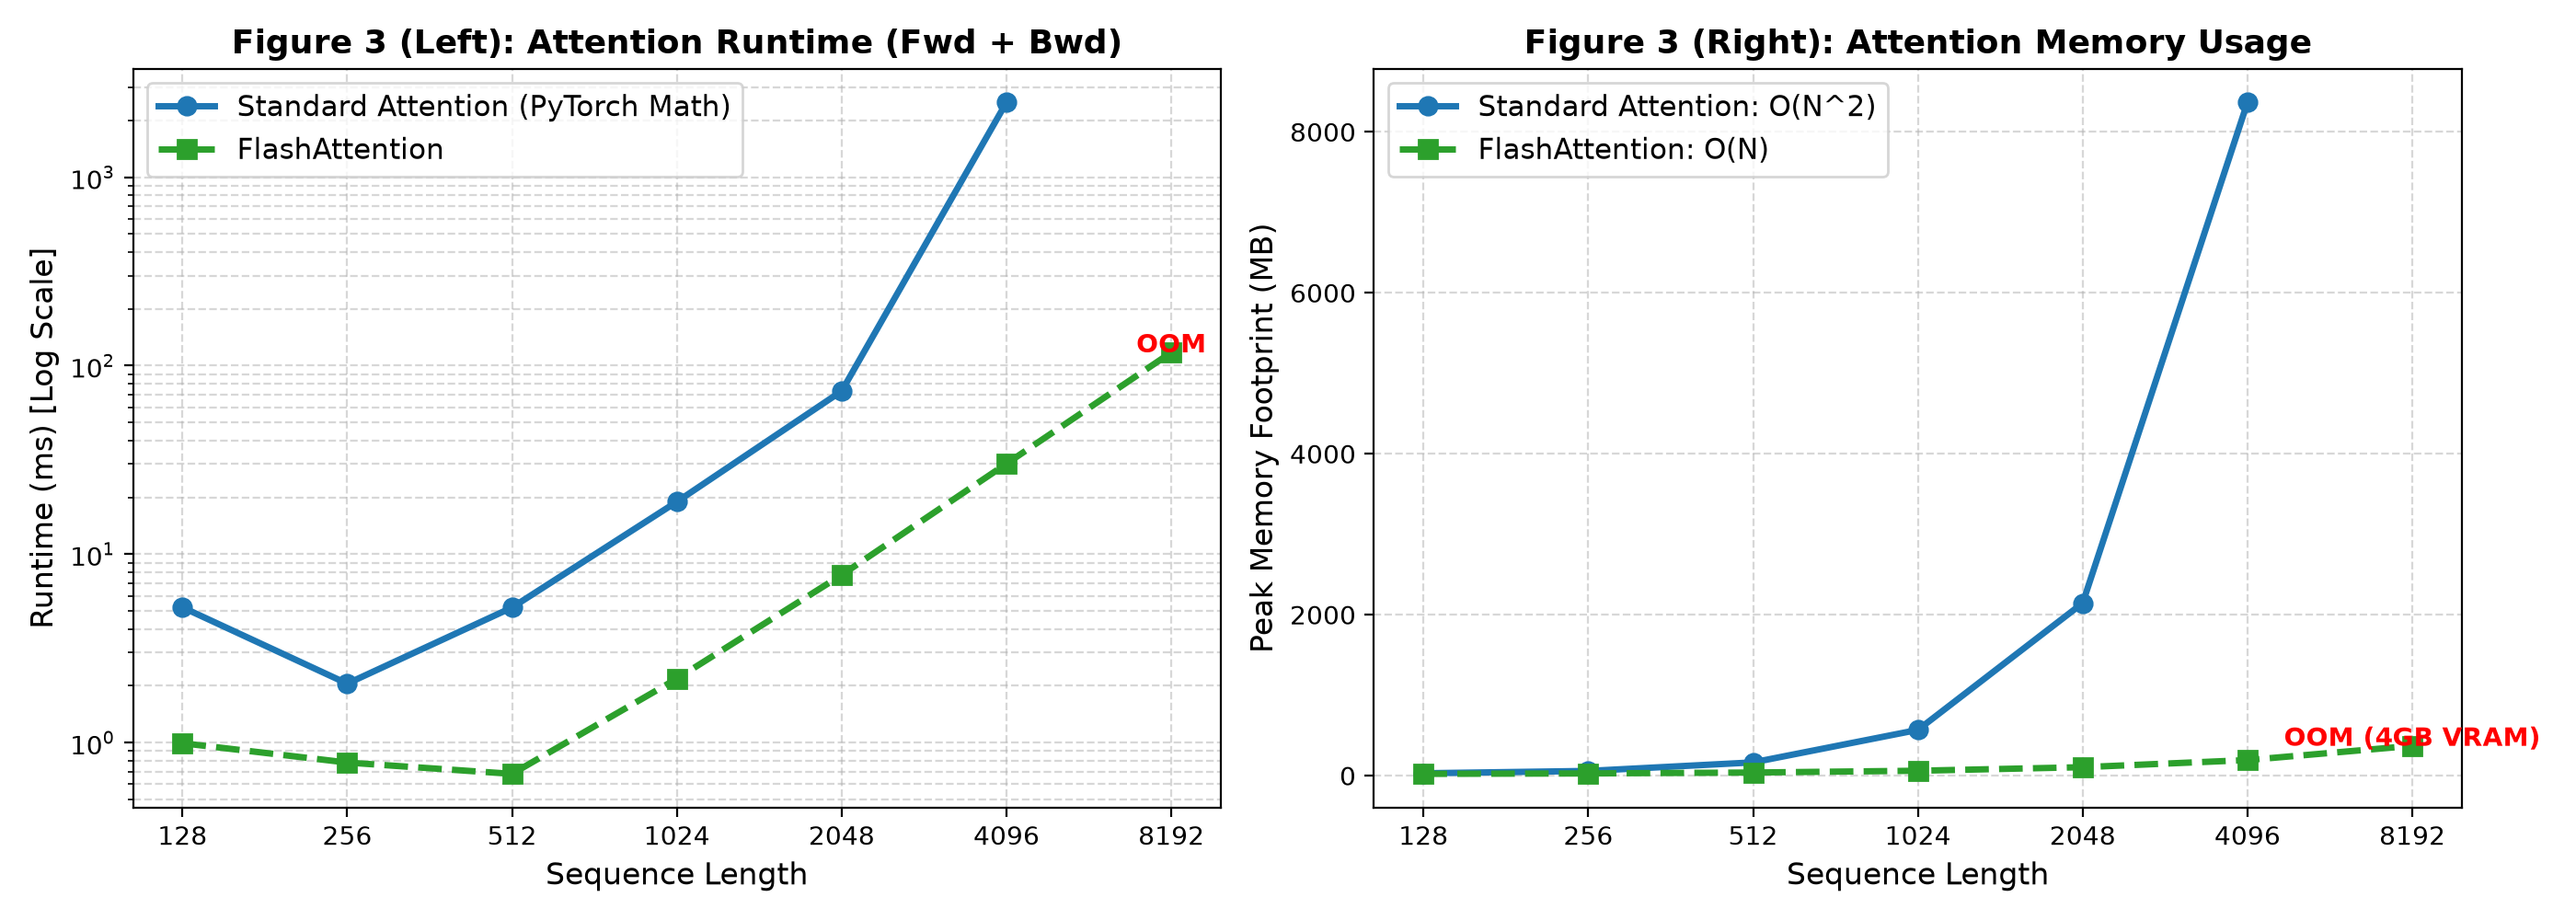
\includegraphics[width=\linewidth]{figure3_reproduction.png}
      \vspace{-0.6em}
      \captionof{figure}{\scriptsize Tái lập Figure 3: Thời gian thực thi (trái) \& Bộ nhớ (phải)}
    \end{center}
  \end{column}

  \begin{column}{0.50\textwidth}
    \begin{block}{Ba Hiện tượng Phần cứng Cốt lõi}
      \begin{enumerate}
        \item \textbf{Chuỗi ngắn ($N \le 512$)}:
          \begin{itemize}
            \item Standard bị overhead khởi chạy nhiều kernel rời rạc và warp under-utilization ($5.21 \text{ ms} \to 2.05 \text{ ms}$).
            \item Flash dùng \textbf{Kernel Fusion} nên độ trễ cực thấp và ổn định ($0.99 \to 0.68 \text{ ms}$).
          \end{itemize}
        \item \textbf{Vùng trung bình ($N = 1024 - 2048$)}:
          \begin{itemize}
            \item Speedup ổn định từ \textbf{8.69$\times \to$ 9.45$\times$}, phản ánh lợi thế cắt giảm I/O HBM.
          \end{itemize}
        \item \textbf{Vách đá hiệu năng tại $N = 4096$}:
          \begin{itemize}
            \item Standard vượt 4GB VRAM $\implies$ kích hoạt Host Memory Paging qua bus PCIe chậm chạp ($73 \text{ ms} \to \mathbf{2496 \text{ ms}}$).
            \item Flash chỉ mất \textbf{30.16 ms} $\implies$ \textbf{Speedup 82.75$\times$}!
          \end{itemize}
      \end{enumerate}
    \end{block}
  \end{column}
\end{columns}
\end{frame}

% ------------------------------------------------------------------------------
% SLIDE 11: PHÂN TÍCH BỘ NHỚ (MEMORY FOOTPRINT)
% ------------------------------------------------------------------------------
\begin{frame}{10. Phân tích Bộ nhớ: Tuyến tính $O(N)$ \& Hóa giải Rào cản OOM}
\begin{columns}[T]
  \begin{column}{0.48\textwidth}
    \begin{center}
      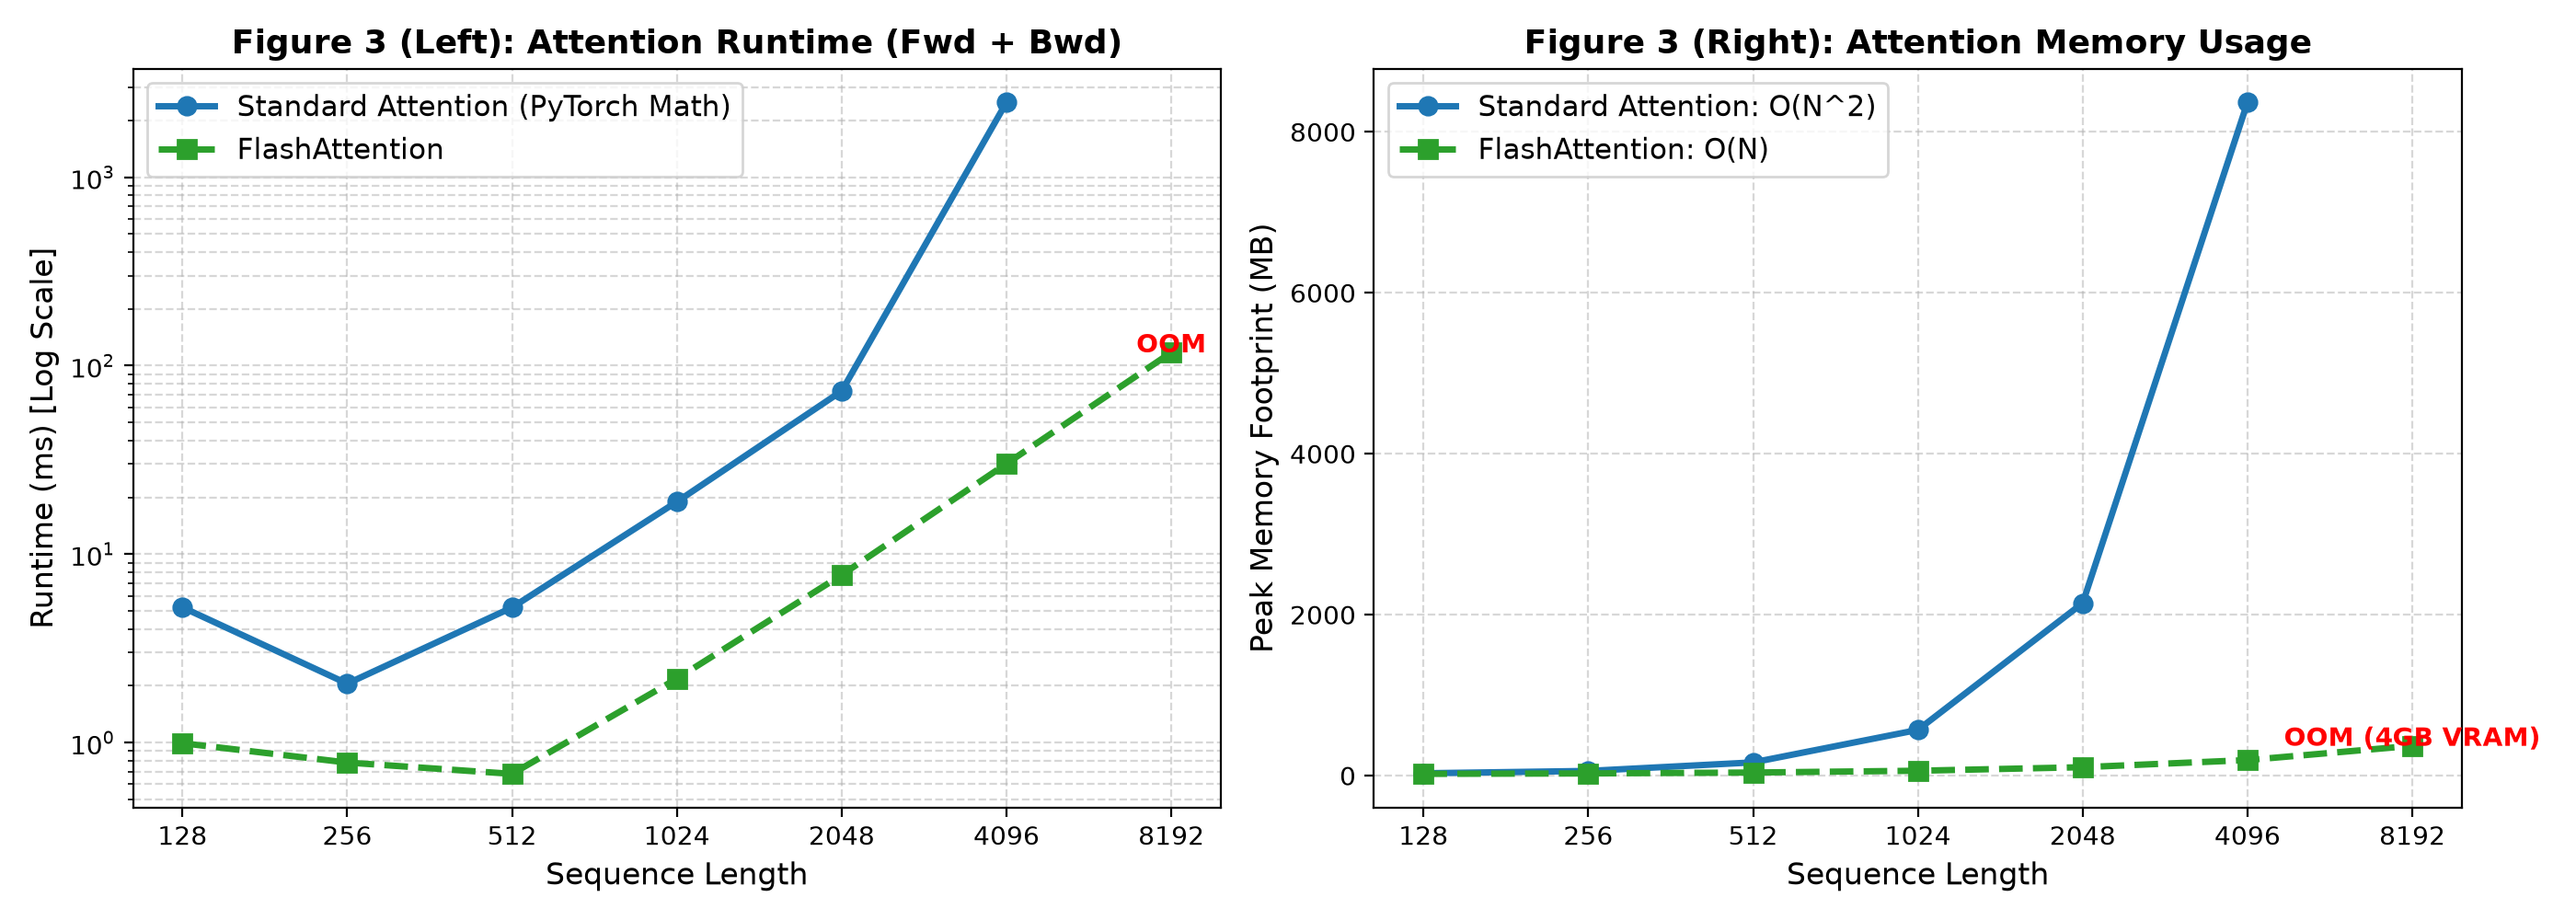
\includegraphics[width=\linewidth]{figure3_reproduction.png}
      \vspace{-0.6em}
      \captionof{figure}{\scriptsize Tái lập Figure 3: Độ dốc bộ nhớ $O(N^2)$ (đỏ) vs $O(N)$ (xanh)}
    \end{center}
  \end{column}

  \begin{column}{0.50\textwidth}
    \begin{block}{Quy luật Tăng trưởng Bộ nhớ VRAM}
      \begin{itemize}
        \item \textbf{Standard Attention tăng trưởng $O(N^2)$}: Bùng nổ theo hàm mũ do phải lưu ma trận $N \times N$ ($164 \text{ MB} \to 2144 \text{ MB} \to 8368 \text{ MB}$).
        \item \textbf{FlashAttention tăng trưởng tuyến tính $O(N)$}: Duy trì độ dốc 1 hoàn hảo trên đồ thị log-log vì chỉ lưu tensor kích thước $N \times d$.
      \end{itemize}
    \end{block}

    \begin{exampleblock}{Tiết kiệm VRAM \& Hóa giải OOM}
      \begin{itemize}
        \item Tại $N=4096$: Tiết kiệm \textbf{43.29$\times$} VRAM (193.3 MB vs 8368.3 MB).
        \item Tại $N=8192$: Standard Attention cần $> 32$ GB bộ nhớ $\implies$ \textbf{CUDA OOM}. FlashAttention chỉ cần \textbf{370.3 MB VRAM} ($< 10\%$ card 4GB)!
      \end{itemize}
    \end{exampleblock}
  \end{column}
\end{columns}
\end{frame}

% ------------------------------------------------------------------------------
% SLIDE 12: BỨC TRANH TIẾN HÓA (FA1 ĐẾN FA4)
% ------------------------------------------------------------------------------
\begin{frame}{11. Bức tranh Tiến hóa: Từ FlashAttention-1 đến FA-2, FA-3 và FA-4}
\begin{center}
\scriptsize
\setlength{\tabcolsep}{3.5pt}
\renewcommand{\arraystretch}{1.1}
\begin{tabular}{lcccc}
\toprule
\textbf{Đặc tính So sánh} & \textbf{FlashAttention-1} & \textbf{FlashAttention-2} & \textbf{FlashAttention-3} & \textbf{FlashAttention-4} \\
\midrule
Năm công bố & 2022 (NeurIPS) & 2023 (ICLR) & 2024 & Đang phát triển \\
Tác giả chính & Tri Dao et al. & Tri Dao & Tri Dao et al. & Open Source / Meta \\
Vòng lặp ngoài & Khối $K, V$ & \textbf{Khối $Q$} & Khối $Q$ & Warp Specialized \\
Chiều song song & Batch, Head & \textbf{Batch, Head, SeqLen} & Batch, Head, SeqLen & Asymmetric Tiled \\
Kỹ thuật then chốt & Tiling, Online Softmax & Warp Partitioning & \textbf{TMA, WGMMA, FP8} & CuTe-DSL, Multi-stage \\
Định dạng số học & FP16, BF16 & FP16, BF16 & FP16, BF16, \textbf{FP8} & FP4, FP8, FP16 \\
Hiệu suất Peak FLOPs & $\sim 35 - 45\%$ & $\sim 55 - 73\%$ & $\sim 75 - 85\%$ & Dự kiến $> 85\%$ \\
\bottomrule
\end{tabular}
\end{center}

\vspace{-0.3em}
\begin{columns}[T]
  \begin{column}{0.48\textwidth}
    \begin{block}{Cải tiến then chốt của FlashAttention-2}
      Đảo vòng lặp ngoài duyệt theo $Q$, giữ vector tích lũy $O_i$ trong thanh ghi (registers) $\implies$ chỉ ghi HBM 1 lần duy nhất, tăng tốc $2\times$ so với FA-1!
    \end{block}
  \end{column}
  \begin{column}{0.48\textwidth}
    \begin{block}{Cải tiến phần cứng của FlashAttention-3}
      Khai thác Tensor Memory Accelerator (TMA) và lệnh Warpgroup GEMM trên Hopper (H100), hỗ trợ định dạng FP8 độ chính xác cao.
    \end{block}
  \end{column}
\end{columns}
\end{frame}

% ------------------------------------------------------------------------------
% SLIDE 13: KẾT LUẬN & ĐÓNG GÓP KHOA HỌC
% ------------------------------------------------------------------------------
\begin{frame}{12. Kết luận \& Đóng góp Khoa học}
\begin{columns}[T]
  \begin{column}{0.32\textwidth}
    \begin{block}{1. Chuyển dịch Mô thức}
      \begin{itemize}
        \item Băng thông bộ nhớ là nút thắt thực sự của AI hiện đại.
        \item Thiết kế thuật toán nhận biết phần cứng (\textbf{IO-Awareness}) vượt trội hơn thuần túy đếm FLOPs.
      \end{itemize}
    \end{block}
  \end{column}

  \begin{column}{0.32\textwidth}
    \begin{exampleblock}{2. Tính Toán Chính xác}
      \begin{itemize}
        \item FlashAttention là thuật toán \textbf{Exact Attention}.
        \item Thực nghiệm chứng minh sai số $\epsilon < 10^{-6}$, bảo toàn 100\% chất lượng mô hình không gây tổn thất.
      \end{itemize}
    \end{exampleblock}
  \end{column}

  \begin{column}{0.32\textwidth}
    \begin{alertblock}{3. Bình dân hóa Long-Context}
      \begin{itemize}
        \item GPU cá nhân 4GB VRAM vẫn chạy tốt chuỗi $N=8192$ (262k tokens).
        \item Đạt gia tốc \textbf{82.75$\times$}, tiết kiệm VRAM \textbf{43.29$\times$}, hóa giải lỗi OOM.
      \end{itemize}
    \end{alertblock}
  \end{column}
\end{columns}

\vspace{0.6em}
\begin{center}
  \large \textbf{\color{NavyBlue}FlashAttention là nền tảng bản lề cho kỷ nguyên LLM Ngữ cảnh Siêu Dài!}
\end{center}
\end{frame}

% ------------------------------------------------------------------------------
% SLIDE 14: Q&A & TÀI LIỆU THAM KHẢO
% ------------------------------------------------------------------------------
\begin{frame}{13. Q\&A \& Tài liệu Tham khảo}
\begin{columns}[T]
  \begin{column}{0.55\textwidth}
    \begin{block}{Tài liệu Tham khảo Cốt lõi}
      \footnotesize
      \begin{enumerate}
        \item Dao, T., et al. (2022). \textbf{FlashAttention: Fast and memory-efficient exact attention with IO-awareness}. \textit{NeurIPS 2022}, 35, 16344--16359.
        \item Dao, T. (2023). \textbf{FlashAttention-2: Faster attention with better parallelism and work partitioning}. \textit{ICLR 2024}.
        \item Dao, T., et al. (2024). \textbf{FlashAttention-3: Fast and accurate attention with asynchrony and low-precision}. \textit{arXiv:2407.08608}.
        \item Milakov, E., \& Gimelshein, N. (2018). \textbf{Online normalizer calculation for softmax}. \textit{arXiv:1805.02867}.
      \end{enumerate}
    \end{block}
  \end{column}

  \begin{column}{0.42\textwidth}
    \begin{exampleblock}{Phiên Hỏi \& Đáp (Q\&A)}
      \centering
      \vspace{0.4em}
      {\Large \textbf{\color{NavyBlue}Cảm ơn Quý Thầy Cô và các Bạn đã Lắng nghe!}}
      \vspace{0.8em}
      
      \textit{Xin mời đặt câu hỏi và đóng góp ý kiến thảo luận!}
      \vspace{0.6em}
      
      \rule{0.8\textwidth}{0.4pt}
      \vspace{0.4em}
      
      \footnotesize
      \textbf{Kho lưu trữ mã nguồn tái lập:}\\
      \texttt{github.com/flash-attention-study}\\
      \texttt{docs/slides/slides.pdf}
    \end{exampleblock}
  \end{column}
\end{columns}
\end{frame}

\end{document}
